\documentclass{article}
\usepackage[letterpaper,top=2cm,bottom=2cm,left=3cm,
            right=3cm,marginparwidth=1.75cm]{geometry}
\usepackage{graphicx}
\begin{document}
\begin{minipage}{0.8\textwidth}
    \centering
    \Large
    \textbf{ECE4144 – GPIO Hands On Assignment}
\end{minipage}\\[1em]
\textbf{1. What registers are necessary to set a GPIO pin and to read a GPIO pin? How does each register
function?}\\[0.5em]
In order to control the GPIOs on the microcontroller, we have to take care of three things: DDR, PORT, and PIN. The DDR sets the direction of the GPIO (1 as output and 0 as input); PORT is used to wire data to the data (1 as high voltage and 0 as low voltage). PIN is used to read the daat to the GPIO (1 as HIGH voltage and 0 as LOW voltage). \\[1em]
\textbf{2. Explain how to set, clear, toggle, or test a bit of a register, without changing the other bits.}\\[0.5em]
To set a specific bit in a register, use the bitwise OR operator:
\begin{verbatim}
    DDRX |= (1 << XX);  // Set bit XX of DDRX (Port X Pin XX as output)
\end{verbatim}
To clear a specific bit in a register (set to 0), use the bitwise AND with the negation:
\begin{verbatim}
    DDRX &= ~(1 << XX);  // Clear bit XX of DDRX (Port X Pin XX as input)
\end{verbatim}
To toggle a specific bit in a register, use the bitwise XOR operator:
\begin{verbatim}
    PORTX ^= (1 << XX);  // Toggle bit XX of PORTX (Toggle state of Port X Pin XX)
\end{verbatim}
To check if a specific bit is set or cleared, use the bitwise AND operator:
\begin{verbatim}
    if (PINX & (1 << XX)) {
        // Pin XX is high
    } else {
        // Pin XX is low
    }
\end{verbatim}
\textbf{3. Enumerate the available GPIO ports/pins available on the playground classic board.}\\[0.5em]
The ATmega32U4 microcontroller used by the Adafruit Circuit Playground provides some GPIO ports (total 26):\\
Port B (PB0–PB7)\\
Port C (PC6, PC7)\\
Port D (PD0–PD7)\\
Port E (PE2, PE6)\\
Port F (PF0, PF1, PF4–PF7)\\[1em]
\textbf{4.a Select and indicate the three pins you choose on your microcontroller board. Is there
any benefit to using specific pins?}\\[0.5em]
For this project, I selected three pins: \#10, \#9 and \#6. The main reason in selecting these threee pins is that they are on the same side on the Playground Circuit Classic. \\[0.5em]
\textbf{4.b Sketch a schematic including the microcontroller, LEDs and any other supporting
electrical components.}\\[0.5em]
\begin{minipage}{\textwidth}
    \centering
    \#10 -------- LED 0 -------- GND\\
    \#9 -------- LED 1 -------- GND\\
    \#6 -------- LED 2 -------- GND\\
\end{minipage}\\[0.5em]
Then we can have the circuit shown in the following image:\\
\begin{minipage}{\textwidth}
    \centering
    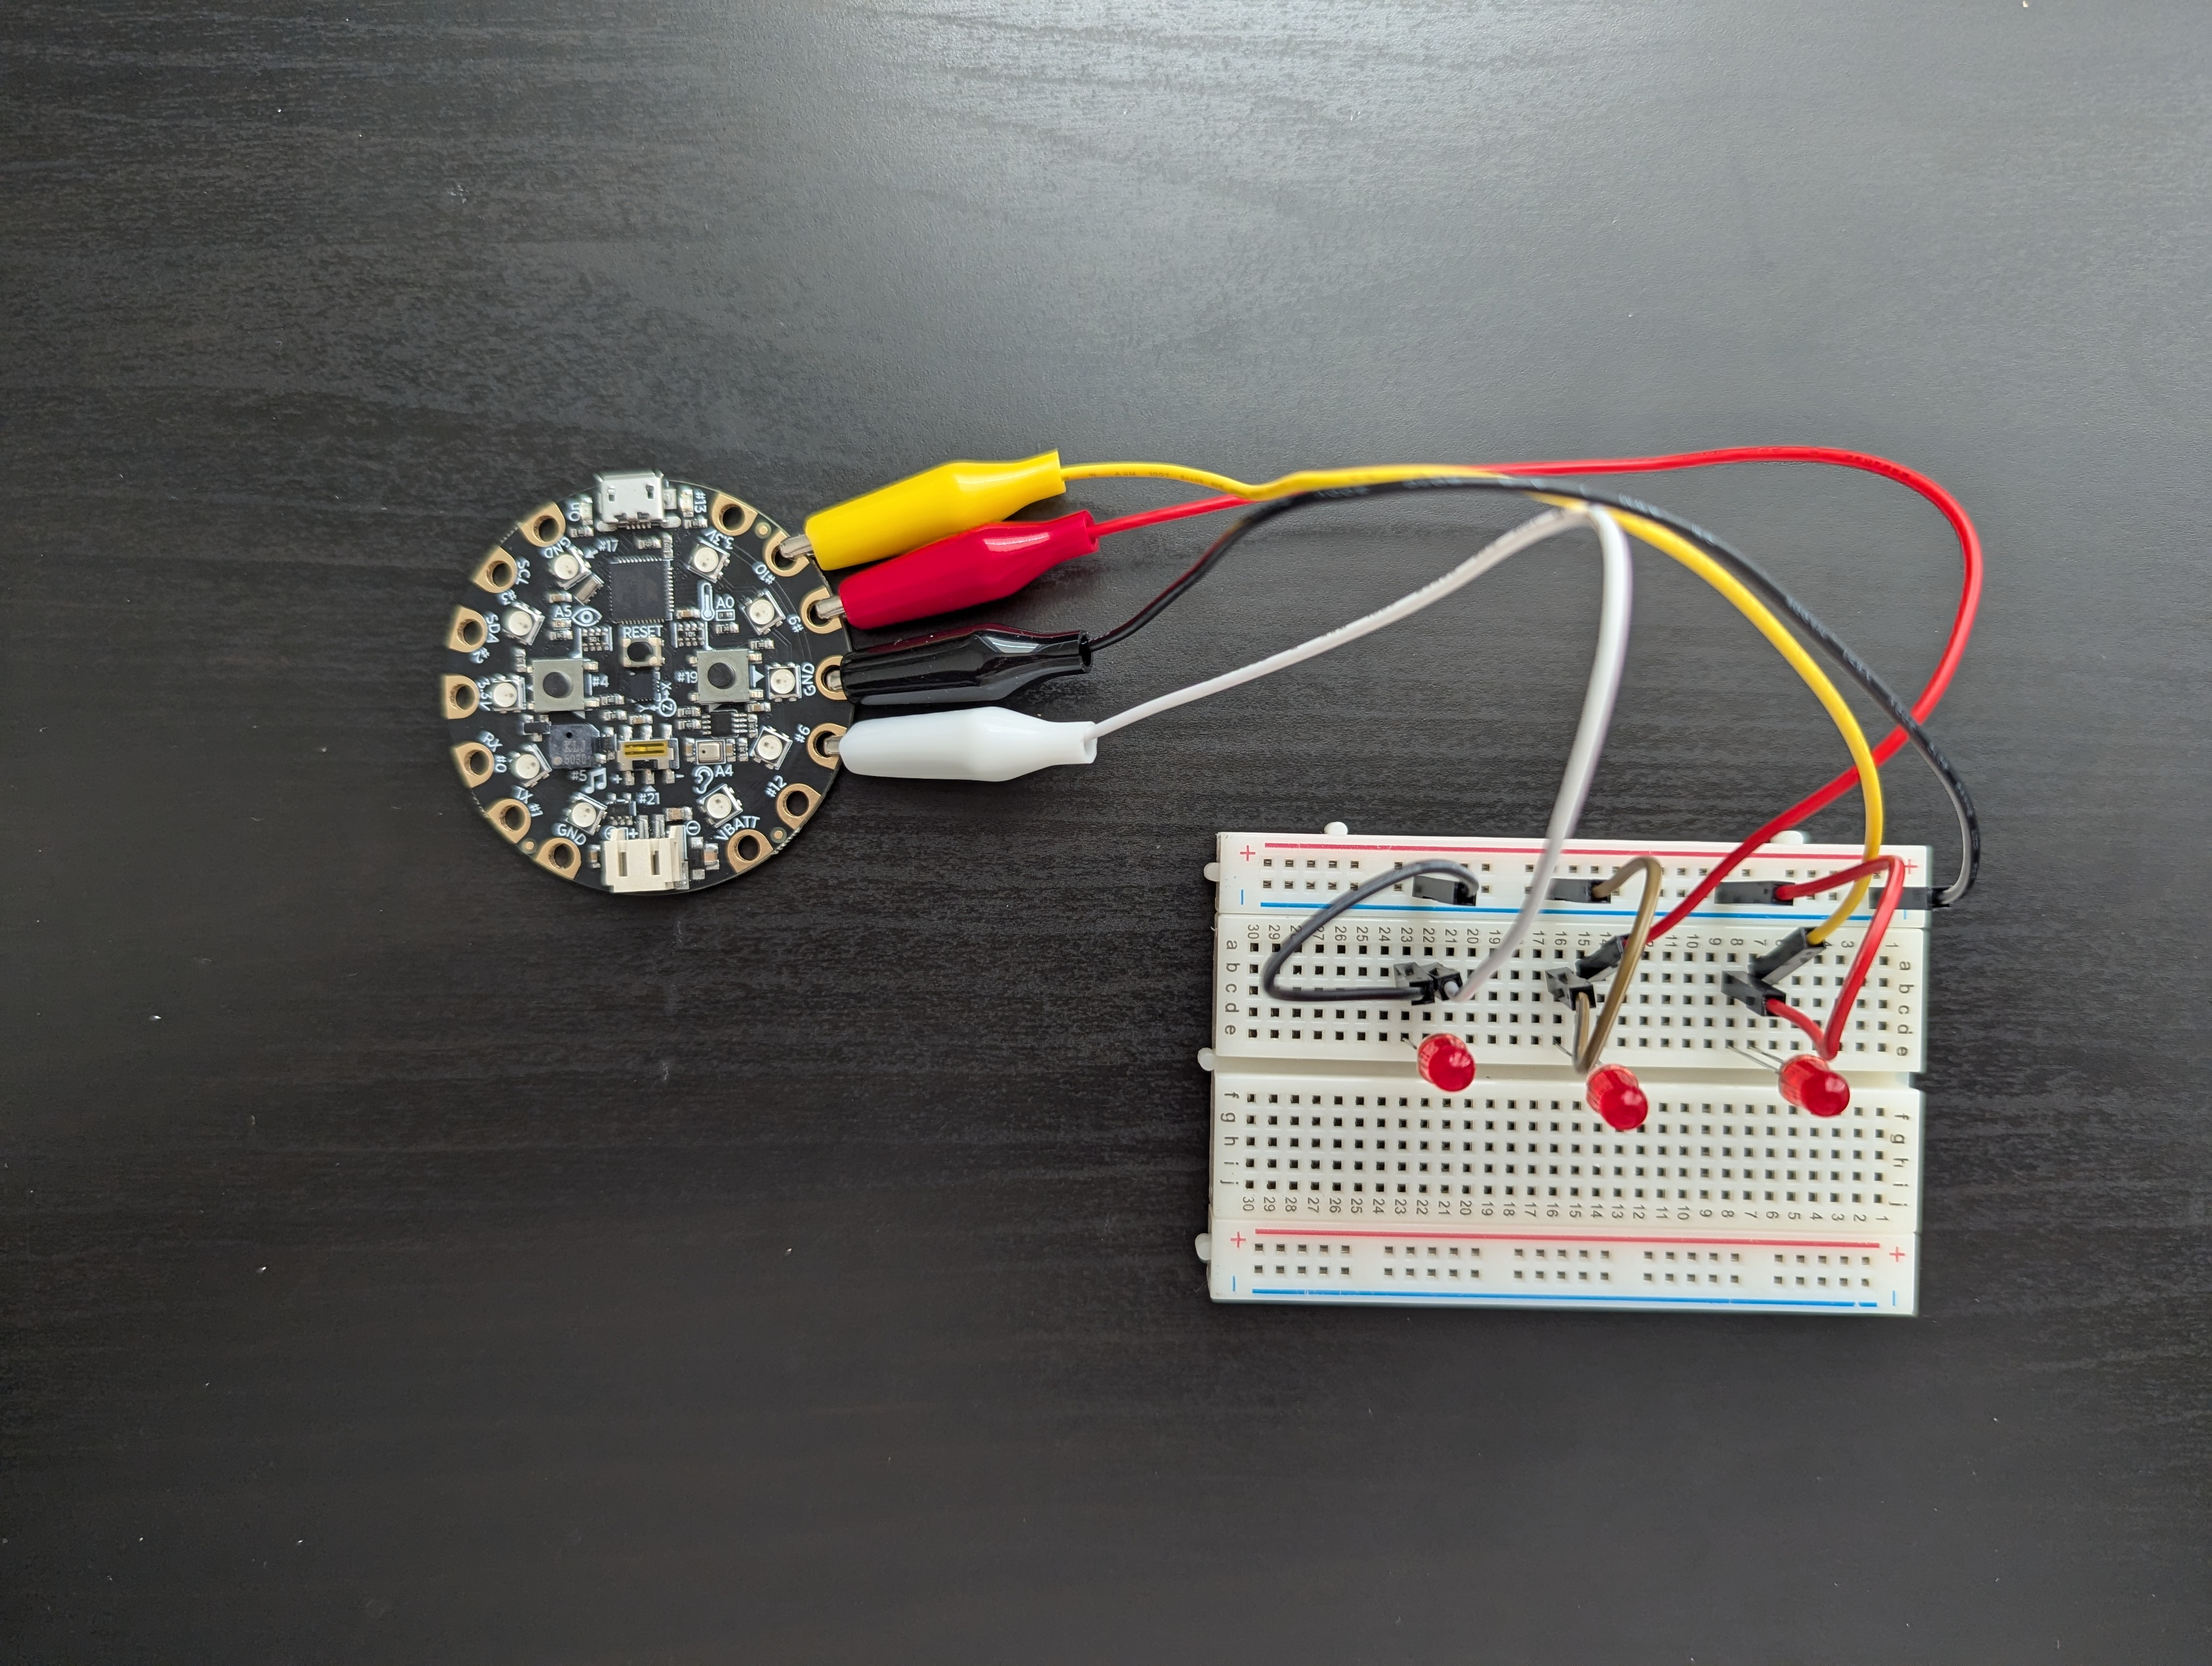
\includegraphics[width = 0.5\textwidth]{circuit.jpg}
\end{minipage}\\[1em]
\textbf{4.c Running Program}
\begin{verbatim}
    #include <Arduino.h>

    // Pin Definitions
    // Digital 10: Port B6
    // Digital 9: Port B5
    // Digital 6: Port D7
    // Left Button: Port D4
    // Right Button: Port F6

    uint8_t looping = 0;
    uint8_t counter = 1;

    void setup() {
    DDRB |= (1 << 6);
    DDRB |= (1 << 5);
    DDRD |= (1 << 7);

    DDRD &= ~(1 << 4);
    DDRF &= ~(1 << 6);

    PORTB &= ~(1 << 6);
    PORTB &= ~(1 << 5);
    PORTD &= ~(1 << 7);
    }

    void loop() {
    if (PIND & (1 << 4)) {
        looping = 1;
        delay(50);
    }

    if (PINF & (1 << 6)) {
        looping = 0;
        delay(50);
    }

    if (looping) {
        PORTB &= ~(1 << 6);
        PORTB &= ~(1 << 5);
        PORTD &= ~(1 << 7);

        if (counter == 1) {
        PORTB |= (1 << 6); // Digital 10 on
        } else if (counter == 2) {
        PORTB |= (1 << 5); // Digital 9 on
        } else if (counter == 3) {
        PORTB |= (1 << 6) | (1 << 5); // Digital 10 and 9 on
        } else if (counter == 4) {
        PORTD |= (1 << 7); // Digital 6 on
        } else if (counter == 5) {
        PORTD |= (1 << 7); // Digital 6 on
        PORTB |= (1 << 6); // Digital 10 on
        } else if (counter == 6) {
        PORTD |= (1 << 7); // Digital 6 on
        PORTB |= (1 << 5); // Digital 9 on
        } else if (counter == 7) {
        PORTB |= (1 << 6) | (1 << 5); // Digital 10 and 9 on
        PORTD |= (1 << 7);            // Digital 6 on
        }

        counter++;
        if (counter > 7) {
        counter = 1;
        }

        delay(500);
    }
    }
\end{verbatim}
The program is also uploaded to the \texttt{hands\_on\_1.cpp} file in the submission. 
\end{document}